\subsubsection{Einflüsse auf die Routenberechnung}
\label{sec:route_explanation_definition}

\begin{figure}[htb!]
    \centering
    \subfloat[1. Prototyp zur Positionierung der \textit{Affordance}]
    {
        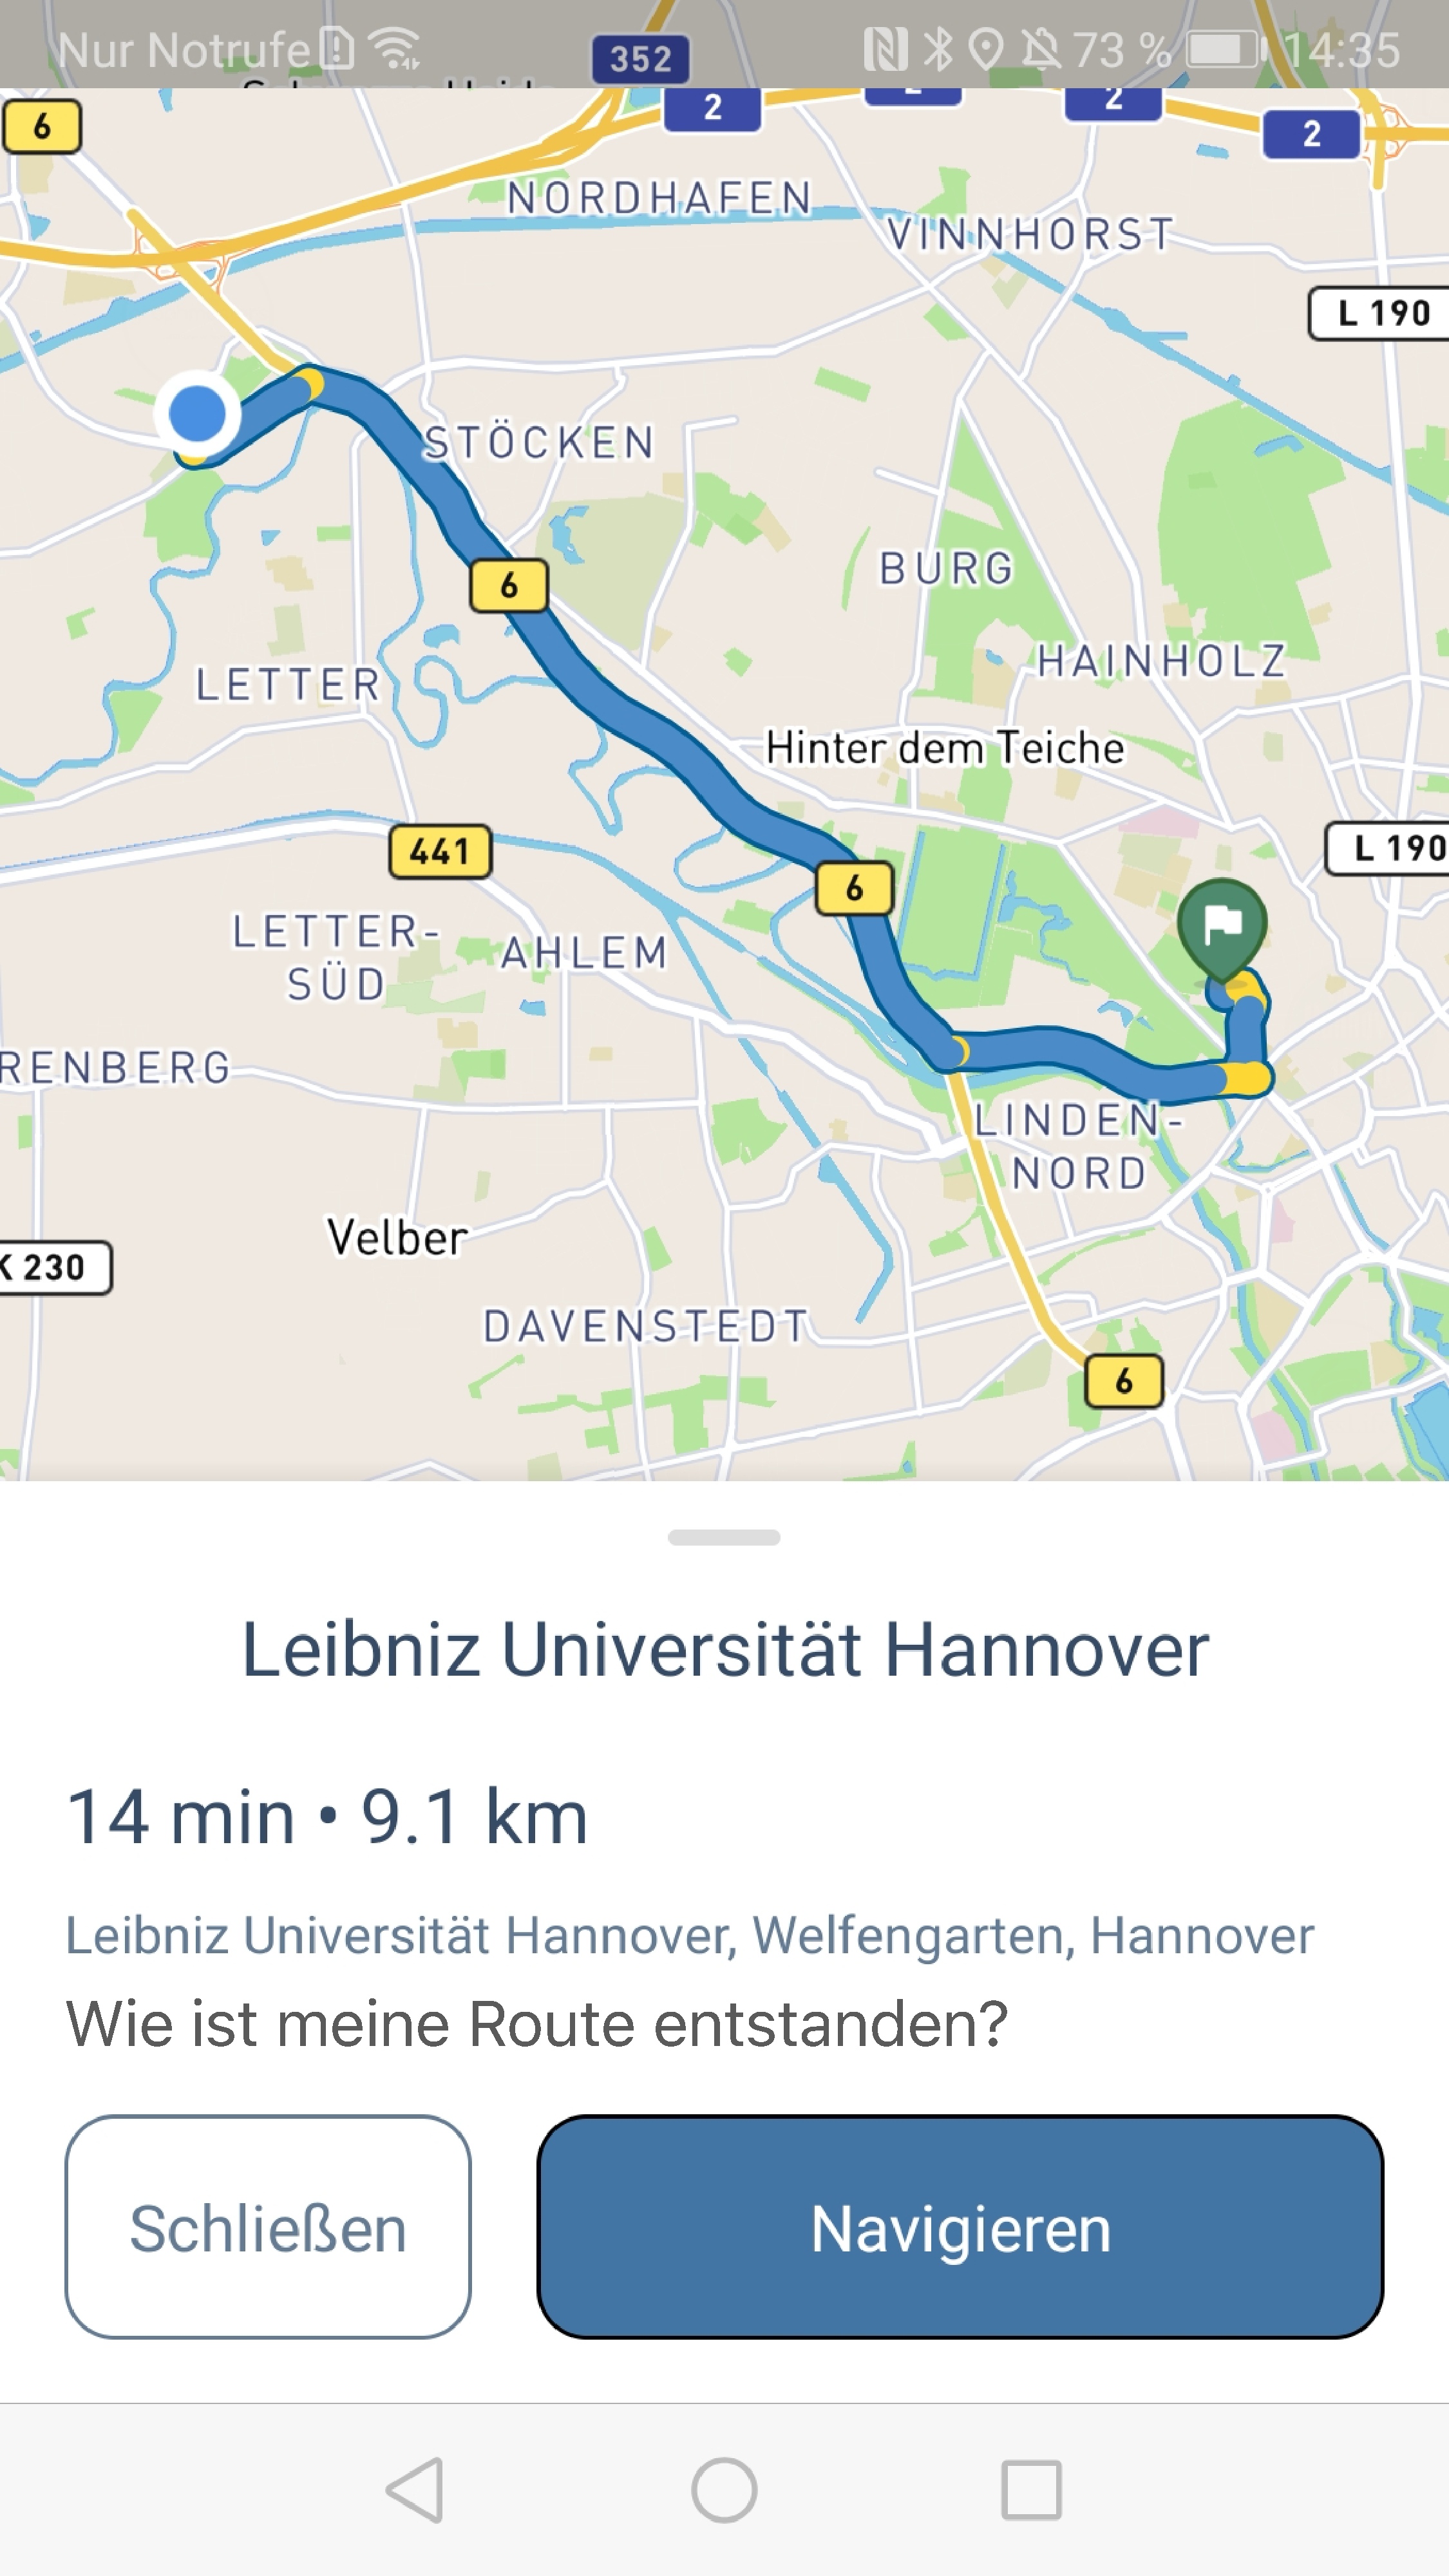
\includegraphics[width=.27\linewidth]{contents/06_model_evaluation/01_integration/res/02_routing_algorithm/prototype_1.pdf}
    }
    \hspace{.055\linewidth}
    \subfloat[Alternativer Prototyp zur Positionierung der \textit{Affordance}]
    {
        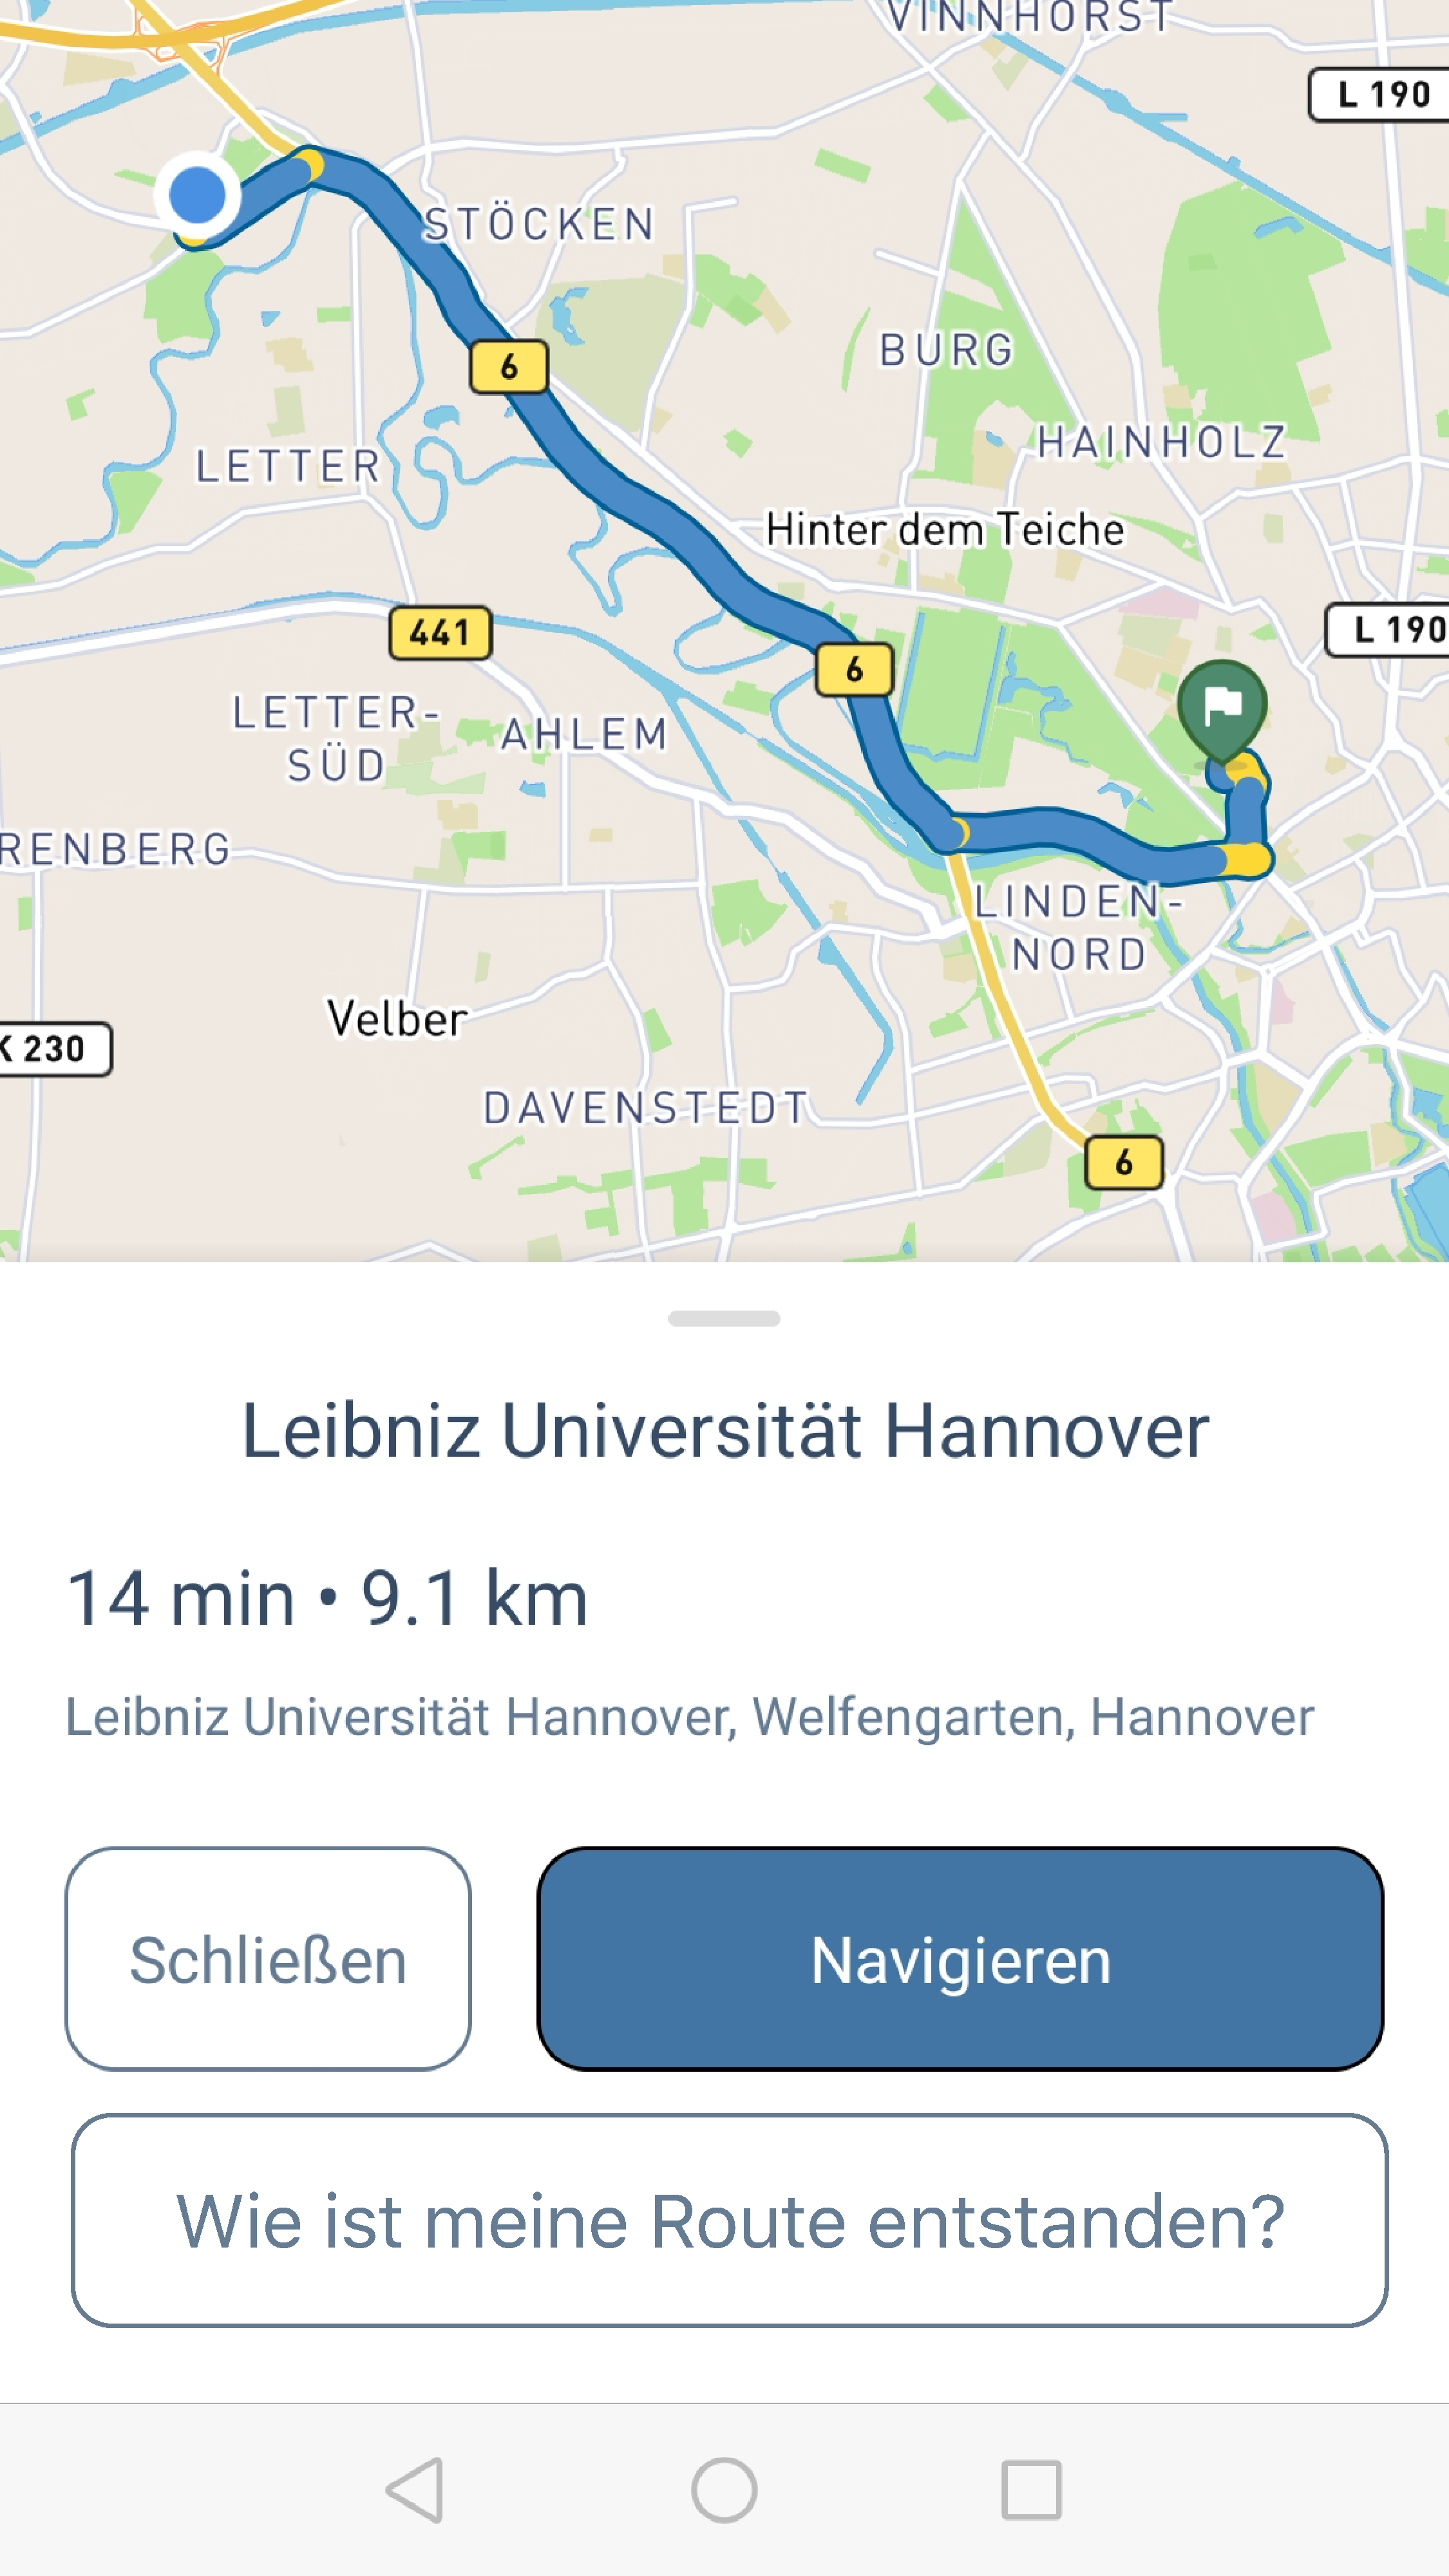
\includegraphics[width=.27\linewidth]{contents/06_model_evaluation/01_integration/res/02_routing_algorithm/prototype_2.pdf}
    }
    \hspace{.055\linewidth}
    \subfloat[Finales Design der kurzen Erklärung]
    {
        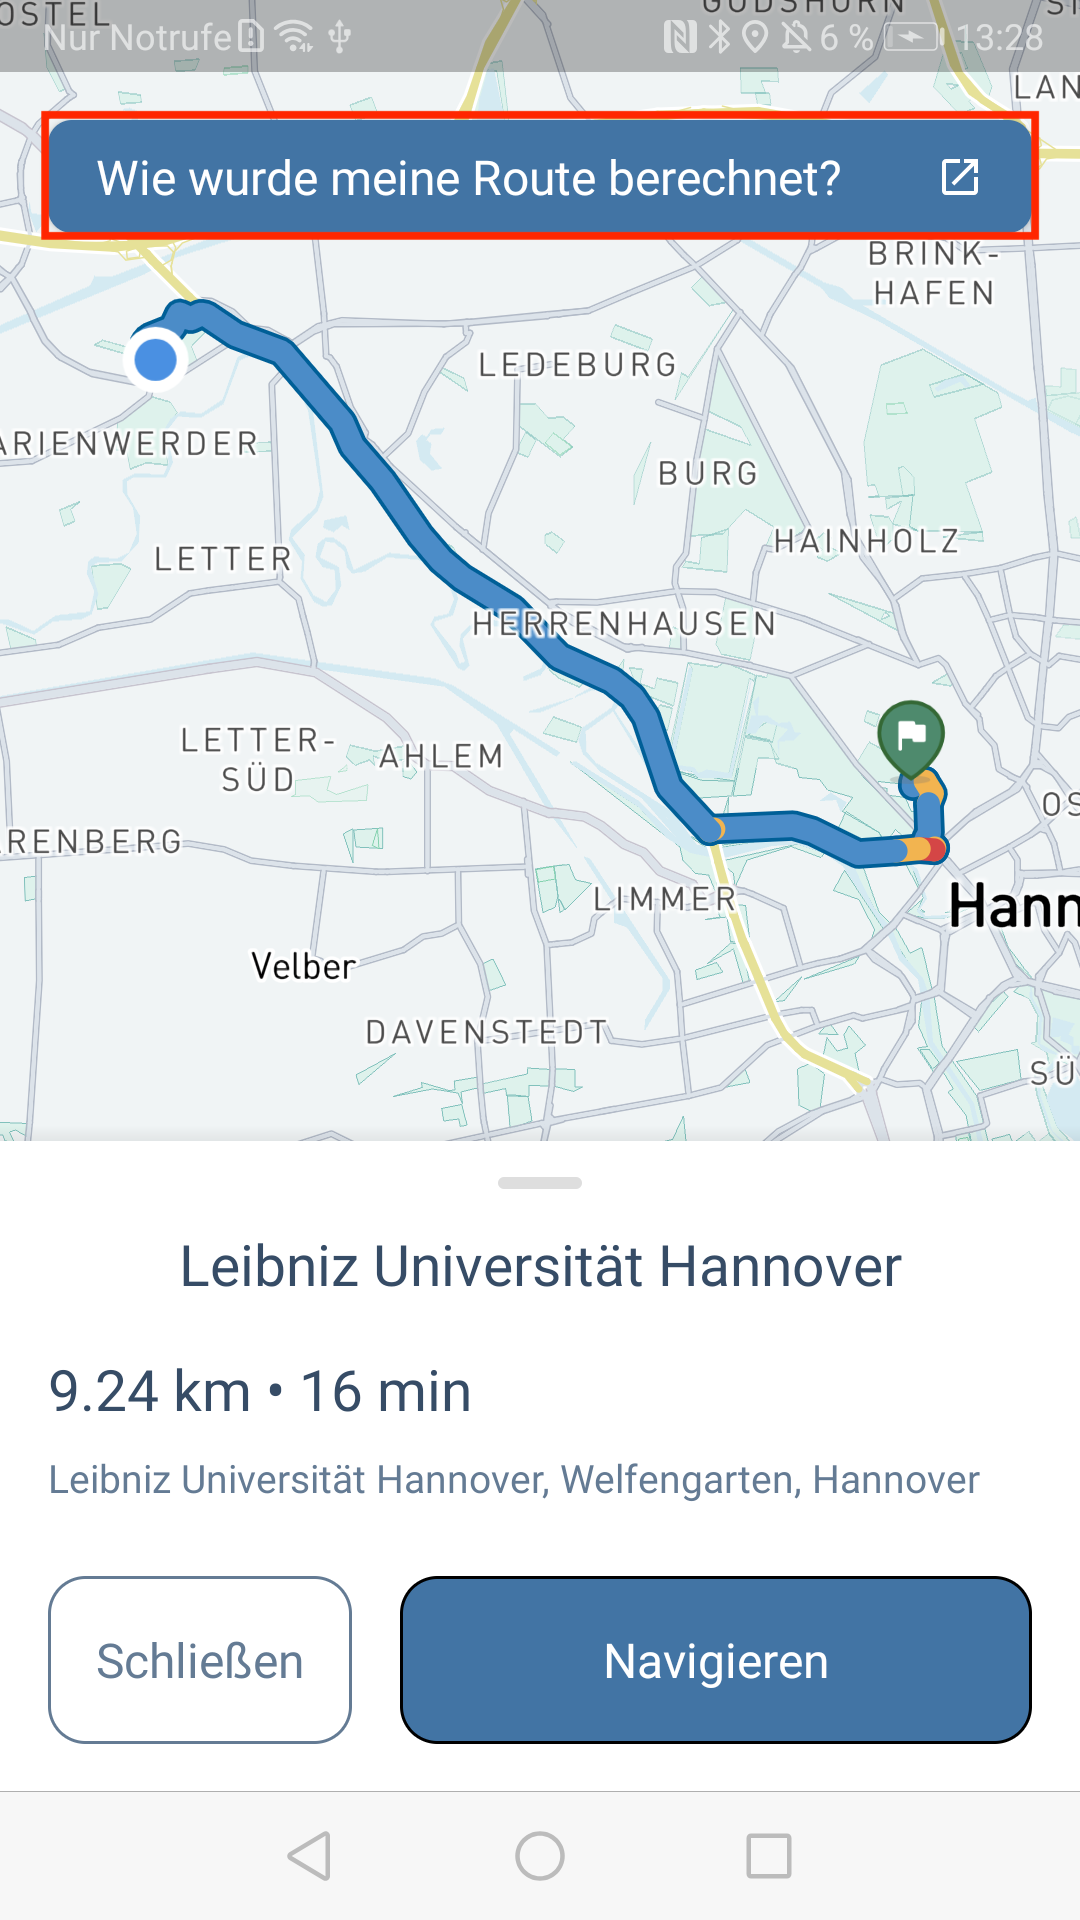
\includegraphics[width=.27\linewidth]{contents/06_model_evaluation/01_integration/res/02_routing_algorithm/final_1.png}
    }
    \caption{Prototyp und finale Designs für die Erklärung zum kollaborativem Routing}
    \label{fig:prototype_routing_explanation}
\end{figure}